\documentclass{scrreprt}

\usepackage{aligned-overset}
\usepackage{amsmath}
\usepackage{amsthm}
\usepackage{amssymb}
\usepackage{bm}
\usepackage[inline, shortlabels]{enumitem}
\usepackage{hyperref}
\usepackage[utf8]{inputenc}
\usepackage{listings}
\usepackage{multicol}
\usepackage{mathtools}
\usepackage{pdflscape}
\usepackage{physics}
\usepackage{polynom}
\usepackage{tabularx}
\usepackage[table]{xcolor}
\usepackage{titling}
\usepackage{fancyhdr}
\usepackage{xfrac}
\usepackage{pgfplots}

\pgfplotsset{compat = newest}
\usepgfplotslibrary{fillbetween}
\usetikzlibrary{arrows, arrows.meta}
\usetikzlibrary{calc}
\usetikzlibrary{patterns}

\author{Karsten Lehmann}
\date{WiSe 2024/25}
\title{Übungsblatt 10\\INF-B-110, Diskrete Strukturen}

\setlength{\parindent}{0pt}

\setlength{\headheight}{26pt}
\pagestyle{fancy}
\fancyhf{}
\lhead{\thetitle}
\rhead{\theauthor}
\lfoot{\thedate}
\rfoot{Seite \thepage}

\newcommand{\ggT}[0]{\text{ggT}}
\DeclarePairedDelimiter{\floor}{\lfloor}{\rfloor}

\begin{document}

\paragraph{Ü 10.1} Durch die folgenden Diagramme sind zwei Graphen definiert:

\begin{minipage}{.45\textwidth}
  \begin{tikzpicture}
    \node[circle, draw, inner sep=0pt, minimum size=1mm,label=right:{1}] (1) at (0,0) {};
    \node[circle, draw, inner sep=0pt, minimum size=1mm,label=left:{2}] (2) at (-1,0) {};
    \node[circle, draw, inner sep=0pt, minimum size=1mm,label=left:{3}] (3) at (-1,-1) {};
    \node[circle, draw, inner sep=0pt, minimum size=1mm,label=left:{4}] (4) at (-1,-2) {};
    \node[circle, draw, inner sep=0pt, minimum size=1mm,label=right:{5}] (5) at (0,-1) {};
    \node[circle, draw, inner sep=0pt, minimum size=1mm,label=below:{6}] (6) at (0,-2) {};
    \node[circle, draw, inner sep=0pt, minimum size=1mm,label=below:{7}] (7) at (1,-2) {};
    \node[circle, draw, inner sep=0pt, minimum size=1mm,label=below:{8}] (8) at (2,-2) {};
    \node[circle, draw, inner sep=0pt, minimum size=1mm,label=left:{9}] (9) at (1.5,-1) {};
    \node[circle, draw, inner sep=0pt, minimum size=1mm,label=right:{10}] (10) at (2,-1) {};
    \node[circle, draw, inner sep=0pt, minimum size=1mm,label=right:{11}] (11) at (2,0) {};
    \node[circle, draw, inner sep=0pt, minimum size=1mm,label=right:{12}] (12) at (3,-2) {};

    \draw (1) -- (2) -- (3) -- (4) -- (6) -- (5) -- (3);
    \draw (5) -- (7);
    \draw (6) -- (7) -- (8) -- (10) -- (11) -- (9) -- (8) -- (12);

    \node at (0.5, -3) {$G_1 = \qty\big(V_1, E_1)$};
  \end{tikzpicture}
\end{minipage}
\begin{minipage}{.45\textwidth}
  \begin{tikzpicture}
    \node[circle, draw, inner sep=0pt, minimum size=1mm,label=below:{1}] (1) at (-1,-2) {};
    \node[circle, draw, inner sep=0pt, minimum size=1mm,label=below:{2}] (2) at (1,-2) {};
    \node[circle, draw, inner sep=0pt, minimum size=1mm,label=above:{3}] (3) at (0,-1) {};
    \node[circle, draw, inner sep=0pt, minimum size=1mm,label=above:{4}] (4) at (-1,0) {};
    \node[circle, draw, inner sep=0pt, minimum size=1mm,label=above:{5}] (5) at (1,0) {};
    \node[circle, draw, inner sep=0pt, minimum size=1mm,label=below:{6}] (6) at (2,-2) {};
    \node[circle, draw, inner sep=0pt, minimum size=1mm,label=above:{7}] (7) at (2,0) {};
    \node[circle, draw, inner sep=0pt, minimum size=1mm,label=below:{8}] (8) at (2.5,-2) {};
    \node[circle, draw, inner sep=0pt, minimum size=1mm,label=above:{9}] (9) at (2.5,0) {};

    \draw (1) -- (2) -- (3) -- (4) -- (5) -- (3) -- (1);
    \draw (6) -- (7);
    \draw (8) -- (9);

    \node at (0.5, -3) {$G_2 = \qty\big(V_2, E_2)$};
  \end{tikzpicture}
\end{minipage}

Geben Sie für beiden Graphen
\begin{itemize}
\item alle Blöcke jeweils durch ein Diagramm an.


  \subparagraph{Lsg.}\phantom{\null}

  \begin{minipage}{.45\textwidth}
    \begin{tikzpicture}
      \draw[fill, green!20] (-0.4,0.2) ellipse (0.6cm and 0.3cm);
      \draw[fill, teal!15] (-1,-0.3) ellipse (0.3cm and 0.5cm);
      \draw[fill, red!20] (2.8,-2) ellipse (0.6cm and 0.3cm);
      \draw[fill, magenta!30] (1.4,-2) ellipse (0.3cm and 0.2cm);
      \draw[fill, blue!20] (1.9, -0.7) ellipse (0.9cm and 1.2cm);
      \begin{scope}[rotate=-12]
        \draw[fill, orange!30] (0,-1.6) ellipse (1.4cm and .7cm);
      \end{scope}

      \node[circle, draw, inner sep=0pt, minimum size=1mm,label=right:{1}] (1) at (0,0.2) {};
      \node[circle, draw, inner sep=0pt, minimum size=1mm,label=above:{2}] (2_1) at (-0.8,0.2) {};
      \node[circle, draw, inner sep=0pt, minimum size=1mm,label=left:{2}] (2_2) at (-1,0) {};
      \node[circle, draw, inner sep=0pt, minimum size=1mm,label=left:{3}] (3_1) at (-1,-0.6) {};
      \node[circle, draw, inner sep=0pt, minimum size=1mm,label=left:{3}] (3_2) at (-1,-1) {};
      \node[circle, draw, inner sep=0pt, minimum size=1mm,label=left:{4}] (4) at (-1,-2) {};
      \node[circle, draw, inner sep=0pt, minimum size=1mm,label=right:{5}] (5) at (0,-1) {};
      \node[circle, draw, inner sep=0pt, minimum size=1mm,label=below:{6}] (6) at (0,-2) {};
      \node[circle, draw, inner sep=0pt, minimum size=1mm,label=below:{7}] (7_1) at (0.8,-2) {};
      \node[circle, draw, inner sep=0pt, minimum size=1mm,label=below:{7}] (7_2) at (1.2,-2) {};
      \node[circle, draw, inner sep=0pt, minimum size=1mm,label=below:{8}] (8_1) at (1.6,-2) {};
      \node[circle, draw, inner sep=0pt, minimum size=1mm,label=below:{8}] (8_2) at (2,-1.8) {};
      \node[circle, draw, inner sep=0pt, minimum size=1mm,label=below:{8}] (8_3) at (2.4,-2) {};
      \node[circle, draw, inner sep=0pt, minimum size=1mm,label=left:{9}] (9) at (1.5,-0.8) {};
      \node[circle, draw, inner sep=0pt, minimum size=1mm,label=right:{10}] (10) at (2,-0.8) {};
      \node[circle, draw, inner sep=0pt, minimum size=1mm,label=right:{11}] (11) at (2,0.2) {};
      \node[circle, draw, inner sep=0pt, minimum size=1mm,label=right:{12}] (12) at (3.2,-2) {};

      \draw (1) -- (2_1);
      \draw (2_2)-- (3_1);
      \draw (3_2)-- (4) -- (6) -- (5) -- (3_2);
      \draw (5) -- (7_1) -- (6);
      \draw (7_2) -- (8_1);
      \draw (8_2) -- (10) -- (11) -- (9) -- (8_2);
      \draw (8_3)-- (12);

      \node at (0.5, -3) {$G_1 = \qty\big(V_1, E_1)$};
    \end{tikzpicture}
  \end{minipage}
  \begin{minipage}{.45\textwidth}
    \begin{tikzpicture}
      \draw[fill, orange!30] (4,-1) ellipse (0.7cm and 1.6cm);
      \draw[fill, green!20] (2.5,-1) ellipse (0.7cm and 1.6cm);
      \draw[fill, blue!20] (0,-0.1) ellipse (1.5cm and 0.8cm);
      \draw[fill, red!20] (0,-1.9) ellipse (1.5cm and 0.8cm);

      \node[circle, draw, inner sep=0pt, minimum size=1mm,label=below:{1}] (1) at (-1,-2) {};
      \node[circle, draw, inner sep=0pt, minimum size=1mm,label=below:{2}] (2) at (1,-2) {};
      \node[circle, draw, inner sep=0pt, minimum size=1mm,label=above:{3}] (3_1) at (0,-0.8) {};
      \node[circle, draw, inner sep=0pt, minimum size=1mm,label=below:{3}] (3_2) at (0,-1.2) {};
      \node[circle, draw, inner sep=0pt, minimum size=1mm,label=above:{4}] (4) at (-1,0) {};
      \node[circle, draw, inner sep=0pt, minimum size=1mm,label=above:{5}] (5) at (1,0) {};
      \node[circle, draw, inner sep=0pt, minimum size=1mm,label=below:{6}] (6) at (2.5,-2) {};
      \node[circle, draw, inner sep=0pt, minimum size=1mm,label=above:{7}] (7) at (2.5,0) {};
      \node[circle, draw, inner sep=0pt, minimum size=1mm,label=below:{8}] (8) at (4,-2) {};
      \node[circle, draw, inner sep=0pt, minimum size=1mm,label=above:{9}] (9) at (4,0) {};

      \draw (1) -- (2) -- (3_2) -- (1);
      \draw (3_1)-- (4) -- (5) -- (3_1);
      \draw (6) -- (7);
      \draw (8) -- (9);

      \node at (0.5, -3) {$G_2 = \qty\big(V_2, E_2)$};
    \end{tikzpicture}
  \end{minipage}

\item den Blockgraphen durch Knoten- und Kantenmenge an und Zeichnen Sie ein
  Diagramm des Blockgraphen.

  \subparagraph{Lsg.} Seien die Blöcke vom Graphen $G_1$ benannt als
  \begin{itemize}
  \item \colorbox{green!20}{$b_1 = \qty\big{1, 2}$}
  \item \colorbox{teal!30}{$b_2 = \qty\big{2, 3}$}
  \item \colorbox{orange!30}{$b_3 = \qty\big{3, 4, 5, 6, 7}$}
  \item \colorbox{magenta!30}{$b_4 = \qty\big{7, 8}$}
  \item \colorbox{blue!20}{$b_5 = \qty\big{8, 9, 10, 11}$}
  \item \colorbox{red!20}{$b_6 = \qty\big{8, 12}$}
  \end{itemize}
  und $\mathcal{B}_1 = \qty\big{b_1, \ldots, b_6}$.
  Nun ist $A_1 = \qty\big{2, 3, 7 8}$ die Menge der Gelenkpunkte von $G_1$ und
  schließlich
  \[
    \qty(A_1 \cup \mathcal{B}_1, \qty{
      \qty\big{2, b_1},
      \qty\big{2, b_2},
      \qty\big{3, b_2},
      \qty\big{3, b_3},
      \qty\big{7, b_3},
      \qty\big{7, b_4},
      \qty\big{8, b_4},
      \qty\big{8, b_5},
      \qty\big{8, b_6}
    })
  \]
  der Blockgraph von $G_1$.

  \newpage
  Seien weiter die Blöcke vom Graphen $G_2$ benannt als
  \begin{itemize}
  \item \colorbox{blue!20}{$b_1 = \qty\big{3, 4, 5}$}
  \item \colorbox{red!20}{$b_2 = \qty\big{1, 2, 3}$}
  \item \colorbox{green!20}{$b_3 = \qty\big{6, 7}$}
  \item \colorbox{orange!30}{$b_4 = \qty\big{8, 9}$}
  \end{itemize}
  und $\mathcal{B}_2 = \qty\big{b_1, \ldots, b_4}$.
  Nun ist $A_2 = \qty\big{3}$ die Menge der Gelenkpunkte von $G_1$ und
  schließlich
  \[
    \qty(A_2 \cup \mathcal{B}_2, \qty{
      \qty\big{3, b_1},
      \qty\big{3, b_2}
    })
  \]
  der Blockgraph von $G_1$.

  Als Diagramme:

  \begin{minipage}{.45\textwidth}
    \begin{tikzpicture}
      \node[circle, draw, inner sep=0pt, minimum size=1mm,label={[black!30!green]left:{$b_1$}}] (b1) at (-1,0) {};
      \node[circle, draw, inner sep=0pt, minimum size=1mm,label=above:{$2$}] (2) at (-0.5,0) {};
      \node[circle, draw, inner sep=0pt, minimum size=1mm,label={[black!30!teal]below:{$b_2$}}] (b2) at (0,0) {};
      \node[circle, draw, inner sep=0pt, minimum size=1mm,label=above:{$3$}] (3) at (0.5,0) {};
      \node[circle, draw, inner sep=0pt, minimum size=1mm,label={[black!30!orange]below:{$b_3$}}] (b3) at (1,0) {};
      \node[circle, draw, inner sep=0pt, minimum size=1mm,label=above:{$7$}] (7) at (1.5,0) {};
      \node[circle, draw, inner sep=0pt, minimum size=1mm,label={[black!10!magenta]below:{$b_4$}}] (b4) at (2,0) {};
      \node[circle, draw, inner sep=0pt, minimum size=1mm,label=below:{$8$}] (8) at (2.5,0) {};
      \node[circle, draw, inner sep=0pt, minimum size=1mm,label={[black!30!blue]above:{$b_5$}}] (b5) at (2.5,0.5) {};
      \node[circle, draw, inner sep=0pt, minimum size=1mm,label={[black!30!red]right:{$b_6$}}] (b6) at (3,0) {};

      \draw (b1) -- (2) -- (b2) -- (3) -- (b3) -- (7) -- (b4) -- (8) -- (b6);
      \draw (8) -- (b5);

      \node at (0.5, -2) {Blockgraph von $G_1$};
    \end{tikzpicture}
  \end{minipage}
  \begin{minipage}{.45\textwidth}
    \begin{tikzpicture}
      \node[circle, draw, inner sep=0pt, minimum size=1mm,label={[black!30!blue]above:{$b_1$}}] (b1) at (-0.5,0.5) {};
      \node[circle, draw, inner sep=0pt, minimum size=1mm,label=left:{$3$}] (3) at (-0.5,0) {};
      \node[circle, draw, inner sep=0pt, minimum size=1mm,label={[black!30!red]below:{$b_2$}}] (b2) at (-0.5,-0.5) {};

      \node[circle, draw, inner sep=0pt, minimum size=1mm,label={[black!30!green]above:{$b_3$}}] (b3) at (0.5,0) {};
      \node[circle, draw, inner sep=0pt, minimum size=1mm,label={[black!30!orange]above:{$b_4$}}] (b4) at (1,0) {};

      \draw (b1) -- (3) -- (b2);

      \node at (0.5, -2) {Blockgraph von $G_2$};
    \end{tikzpicture}
  \end{minipage}

\end{itemize}


\paragraph{Ü 10.2} Beweisen Sie (zum Beispiel mit der Methode der vollständigen
Induktion), dass der Blockgraph eines beliebigen zusammenhängenden Graphen
$G = \qty\big(V, E)$ zusammenhängend ist.

\subparagraph{Lsg.} Durch vollständige Induktion:

\textbf{Behauptung:}
\[
  P\qty\big(n) \colon \text{Falls ein Graph $G$ mit $n$ Blöcken zusammenhängend
    ist, so ist auch sein Blockgraph $G_B$ zusammenhängend}
\]

\textbf{Induktionsanfang:} Die Aussagen $P\qty\big(0)$ und $P\qty\big(1)$ sind trivial.

Sei nun $P\qty\big(n)$ für ein beliebiges $n \in \mathbb{N}$ mit $n \leq 1$ wahr (Induktionsvoraussetzung).

\textbf{Induktionsschritt:} Es wird $P\qty\big(n + 1)$ betrachtet.
Sei $G$ ein zusammenhängender Graph mit $n + 1$ Blöcken.
Aus der Vorlesung ist bereits bekannt, dass $G_B$ ein Wald ist (Proposition 64).

Nun ist $G$ zusammenhängend mit mindestens zwei Blöcken, somit hat $G_B$
mindestens eine Kante und somit auch mindestens ein Blatt.
Sei nun $B$ ein Blatt in $G_B$ und $c$ der Gelenkpunkt in dem Blatt $B$.

Betrachte nun $G' = G \setminus B \cup \qty\big(c)$.
Dann ist $G'$ zusammenhängend, da der Gelenkpunkt nicht entnommen wurde und nach
der Induktionsvoraussetzung auch $G'_B$ zusammenhängend.

Fügt man nun das Blatt wieder ein, sieht man dass auch $G_B$ zusammenhängend ist
und aus dem Satz über die Vollständige Induktion folgt $P\qty\big(n)$ für alle
$n \in \mathbb{N}$.

\newpage
\paragraph{Ü 10.3} Finden Sie alle zusammenhängenden Graphen, die zu ihrem
Blockgraphen isomorph sind.

\subparagraph{Lsg.} Nach Ü 10.2 ist der Blockgraph $G_B$ eines zusammenhängenden
Graphen $G$ ebenfalls zusammenhängend.
Nun ist ein Blockgraph nach der Vorlesung ein Wald und ein zusammenhängender Wald
ein Baum.
Somit muss $G$ - um isomorph zu seinem Blockgraph $G_B$ sein zu können -
ebenfalls ein Baum sein.

Sei nun ein Graph $G = \qty\big(V, E)$ isomorph zu seinem Blockgraphen $G_B$.
mit $\abs{V} = n$.


$\Rightarrow$ es gibt $n - 1$ Blöcke in dem Graphen.

$\Rightarrow$ es darf nur einen Gelenkpunkt geben, da jeder Block ein Knoten im
Blockgraphen wird und der Blockgraph andernfalls mehr als $n$ Knoten hätte.

Somit sind die Graphen, die isomorph zu ihrem Blockgraphen sind sternförmig, wie
zum Beispiel \\

\begin{tikzpicture}
  \node[circle, draw, inner sep=0pt, minimum size=1mm] (1) at (0,0) {};
  \node[circle, draw, inner sep=0pt, minimum size=1mm] (2) at (0,1) {};
  \node[circle, draw, inner sep=0pt, minimum size=1mm] (3) at ($({-sqrt(3)/2},-0.5)$) {};
  \node[circle, draw, inner sep=0pt, minimum size=1mm] (4) at ($({sqrt(3)/2},-0.5)$) {};

  \draw (2) -- (1);
  \draw (3) -- (1);
  \draw (4) -- (1);

  \node[circle, draw, inner sep=0pt, minimum size=1mm] (5) at (3,0) {};
  \node[circle, draw, inner sep=0pt, minimum size=1mm] (6) at (2,0) {};
  \node[circle, draw, inner sep=0pt, minimum size=1mm] (7) at (3,-1) {};
  \node[circle, draw, inner sep=0pt, minimum size=1mm] (8) at (4,0) {};
  \node[circle, draw, inner sep=0pt, minimum size=1mm] (9) at (3,1) {};

  \draw (5) -- (6);
  \draw (5) -- (7);
  \draw (5) -- (8);
  \draw (5) -- (9);
\end{tikzpicture}

\paragraph{Ü 10.4}
\begin{enumerate}[(a)]
\item Untersuchen Sie die folgenden Graphen darauf, ob sie zweifach
  zusammenhängend sind.
  Geben Sie, wenn möglich, eine Ohrendekomposition an.

  \begin{minipage}{.24\textwidth}
    \begin{tikzpicture}
      \node[circle, draw, inner sep=0pt, minimum size=1mm,label=below:{1}] (1) at (0,0) {};
      \node[circle, draw, inner sep=0pt, minimum size=1mm,label=below:{2}] (2) at (2,0) {};
      \node[circle, draw, inner sep=0pt, minimum size=1mm,label=right:{3}] (3) at (2,2) {};
      \node[circle, draw, inner sep=0pt, minimum size=1mm,label=above:{4}] (4) at (1,2.5) {};
      \node[circle, draw, inner sep=0pt, minimum size=1mm,label=left:{5}] (5) at (0,2) {};

      \draw (3) -- (1) -- (5) -- (4) -- (3) -- (2) -- (5);

      \node at (0.5, -1) {$G_1$};
    \end{tikzpicture}
  \end{minipage}
  \begin{minipage}{.24\textwidth}
    \begin{tikzpicture}
      \node[circle, draw, inner sep=0pt, minimum size=1mm,label=below:{1}] (1) at (1,0) {};
      \node[circle, draw, inner sep=0pt, minimum size=1mm,label=right:{2}] (2) at (2,2) {};
      \node[circle, draw, inner sep=0pt, minimum size=1mm,label=above:{3}] (3) at (1,2.5) {};
      \node[circle, draw, inner sep=0pt, minimum size=1mm,label=left:{4}] (4) at (0,2) {};
      \node[circle, draw, inner sep=0pt, minimum size=1mm,label=right:{5}] (5) at (1,1) {};

      \draw (1) -- (2) -- (3) -- (4) -- (1);
      \draw (4) -- (2);
      \draw (3) -- (5);

      \node at (0.5, -1) {$G_2$};
    \end{tikzpicture}
  \end{minipage}
  \begin{minipage}{.24\textwidth}
    \begin{tikzpicture}[scale=.9]
      \node[circle, draw, inner sep=0pt, minimum size=1mm,label=below:{1}] (1) at (0,0) {};
      \node[circle, draw, inner sep=0pt, minimum size=1mm,label=right:{2}] (2) at ($({sqrt(3)/2}, 0.5)$) {};
      \node[circle, draw, inner sep=0pt, minimum size=1mm,label=right:{3}] (3) at ($({sqrt(3)/2}, 1.5)$) {};
      \node[circle, draw, inner sep=0pt, minimum size=1mm,label=above:{4}] (4) at (0, 2) {};
      \node[circle, draw, inner sep=0pt, minimum size=1mm,label=left:{5}] (5) at ($({-sqrt(3)/2}, 1.5)$) {};
      \node[circle, draw, inner sep=0pt, minimum size=1mm,label=left:{6}] (6) at ($({-sqrt(3)/2}, 0.5)$) {};

      \draw (5) -- (4) -- (3) -- (2) -- (1) -- (6) -- (5) -- (2);
      \draw (3) -- (6);
      \draw (4) -- (1);

      \node at (0.5, -1) {$G_3$};
    \end{tikzpicture}
  \end{minipage}
  \begin{minipage}{.24\textwidth}
    \begin{tikzpicture}[scale=.9]
      \node[circle, draw, inner sep=0pt, minimum size=1mm,label=below:{1}] (1) at (1,0) {};
      \node[circle, draw, inner sep=0pt, minimum size=1mm,label=right:{2}] (2) at (1.5,0.5) {};
      \node[circle, draw, inner sep=0pt, minimum size=1mm,label=right:{3}] (3) at (1,1) {};
      \node[circle, draw, inner sep=0pt, minimum size=1mm,label=right:{4}] (4) at (1,1.5) {};
      \node[circle, draw, inner sep=0pt, minimum size=1mm,label=right:{5}] (5) at (1.5,2) {};
      \node[circle, draw, inner sep=0pt, minimum size=1mm,label=above:{6}] (6) at (1,2.5) {};
      \node[circle, draw, inner sep=0pt, minimum size=1mm,label=above:{7}] (7) at (0.5,1.25) {};
      \node[circle, draw, inner sep=0pt, minimum size=1mm,label=above:{8}] (8) at (0,1.5) {};
      \node[circle, draw, inner sep=0pt, minimum size=1mm,label=below:{9}] (9) at (0,1) {};

      \draw (3) -- (1) -- (2) -- (3) -- (7) -- (9) -- (8) -- (7) -- (4) -- (5) -- (6) -- (4);

      \node at (0.5, -1) {$G_4$};
    \end{tikzpicture}
  \end{minipage}

  \subparagraph{Lsg.} $G_1$ ist zweifach zusammenhängend mit einer
  Beispieldekomposition

  \begin{tikzpicture}
    \node[circle, draw, inner sep=0pt, minimum size=1mm,label=below:{1}] (1) at (0,0) {};
    \node[circle, draw, inner sep=0pt, minimum size=1mm,label=below:{2}] (2) at (1,0) {};
    \node[circle, draw, inner sep=0pt, minimum size=1mm,label=right:{3}] (3) at (1,0.75) {};
    \node[circle, draw, inner sep=0pt, minimum size=1mm,label=above:{4}] (4) at (0.5,1) {};
    \node[circle, draw, inner sep=0pt, minimum size=1mm,label=left:{5}] (5) at (0,0.75) {};

    \draw (3) -- (1) -- (5) -- (4) -- (3) -- (1);
    \draw[red] (5) -- (2) -- (3);
  \end{tikzpicture}

  $G_2$ hat den Knoten 3 als Gelenkpunkt und ist somit nicht zweifach zusammenhängend.

  \newpage
  $G_3$ ist zweifach zusammenhängend mit einer Dekomposition

  \begin{tikzpicture}
    \node[circle, draw, inner sep=0pt, minimum size=1mm,label=below:{1}] (1) at (0,0) {};
    \node[circle, draw, inner sep=0pt, minimum size=1mm,label=right:{2}] (2) at ($({sqrt(3)/4}, 0.25)$) {};
    \node[circle, draw, inner sep=0pt, minimum size=1mm,label=right:{3}] (3) at ($({sqrt(3)/4}, 0.75)$) {};
    \node[circle, draw, inner sep=0pt, minimum size=1mm,label=above:{4}] (4) at (0, 1) {};
    \node[circle, draw, inner sep=0pt, minimum size=1mm,label=left:{5}] (5) at ($({-sqrt(3)/4}, 0.75)$) {};
    \node[circle, draw, inner sep=0pt, minimum size=1mm,label=left:{6}] (6) at ($({-sqrt(3)/4}, 0.25)$) {};

    \draw[red] (6) -- (5) -- (4) -- (3) -- (2) -- (1) -- (6);
    \draw[blue] (1) -- (4);
    \draw[green] (2) -- (5);
    \draw[orange] (3) -- (6);
  \end{tikzpicture}

  $G_4$ hat die Gelenkpunkte $3, 4, 7$ und ist somit nicht zweifach
  zusammenhängend.

\item Bestimmen Sie für alle bipartiten, d.h. 2-färbbaren, Graphen aus (a) die
  Partitionsklassen der Knotenmenge (auch Farbklassen genannt).

  \subparagraph{Lsg}\phantom{\null}

    \begin{minipage}{.24\textwidth}
    \begin{tikzpicture}
      \node[circle, draw, inner sep=0pt, minimum size=1mm,label={[black!30!red]below:{1}}] (1) at (0,0) {};
      \node[circle, draw, inner sep=0pt, minimum size=1mm,label={[black!30!red]below:{2}}] (2) at (2,0) {};
      \node[circle, draw, inner sep=0pt, minimum size=1mm,label={[black!30!blue]right:{3}}] (3) at (2,2) {};
      \node[circle, draw, inner sep=0pt, minimum size=1mm,label={[black!30!red]above:{4}}] (4) at (1,2.5) {};
      \node[circle, draw, inner sep=0pt, minimum size=1mm,label={[black!30!blue]left:{5}}] (5) at (0,2) {};

      \draw (3) -- (1) -- (5) -- (4) -- (3) -- (2) -- (5);

      \node at (0.5, -1) {$G_1$};
    \end{tikzpicture}
  \end{minipage}
  \begin{minipage}{.24\textwidth}
    \begin{tikzpicture}[scale=.9]
      \node[circle, draw, inner sep=0pt, minimum size=1mm,label={[black!30!red]below:{1}}] (1) at (0,0) {};
      \node[circle, draw, inner sep=0pt, minimum size=1mm,label={[black!30!blue]right:{2}}] (2) at ($({sqrt(3)/2}, 0.5)$) {};
      \node[circle, draw, inner sep=0pt, minimum size=1mm,label={[black!30!red]right:{3}}] (3) at ($({sqrt(3)/2}, 1.5)$) {};
      \node[circle, draw, inner sep=0pt, minimum size=1mm,label={[black!30!blue]above:{4}}] (4) at (0, 2) {};
      \node[circle, draw, inner sep=0pt, minimum size=1mm,label={[black!30!red]left:{5}}] (5) at ($({-sqrt(3)/2}, 1.5)$) {};
      \node[circle, draw, inner sep=0pt, minimum size=1mm,label={[black!30!blue]left:{6}}] (6) at ($({-sqrt(3)/2}, 0.5)$) {};

      \draw (5) -- (4) -- (3) -- (2) -- (1) -- (6) -- (5) -- (2);
      \draw (3) -- (6);
      \draw (4) -- (1);

      \node at (0.5, -1) {$G_3$};
    \end{tikzpicture}
  \end{minipage}

\end{enumerate}

\paragraph{Ü 10.5} In einem Sprachkurs nehmen 9 Leute teil.
Alle schicken zu drei anderen des Kurses je eine Postkarte.
Kann es sein, dass alle genau von denjenigen Postkarten bekommen, an die sie die
Postkarten geschickt haben?

\subparagraph{Lsg} Wenn man das Briefversenden als Graph darstellt, dann ist
jeder Knoten ein Teilnehmer und zwei Knoten haben eine Kante, wenn sich die
Teilnehmer gegenseitig einen Brief schicken.

Nun hat jeder Knoten genau Grad 3 und somit
$\abs{E} = \frac{9 \cdot 3}{2} \notin \mathbb{N}$.
\end{document}
